\subsection{The Usual, Spherical \Luscher's Formula}\label{sec:spherical}


Here we present a $D$-dimensional derivation of \Luscher's formula that roughly follows \Ref{Beane:2003da}, although the technology and sophistication of the finite-volume formalism has grown substantially \todo{cite cite cite}\cite{Zhu:2019dho}.

The starting point are interactions given by a tower of derivative contact operators such that the tree amplitude in the center of mass frame is given by
\begin{equation}
    V(p) = + i\sum_n C_{2n}(\Lambda) p^{2n}
\end{equation}
where $p$ denotes the relative momentum of incoming nucleons and the interaction strengths $ C_{2n}(\Lambda)$ depend on the regulator $\Lambda$ and carry spatial-dimension-dependent units.
The scattering amplitude is given by the bubble sum depicted in \Figref{bubbleSum}.

\begin{figure}[ht!]
\center
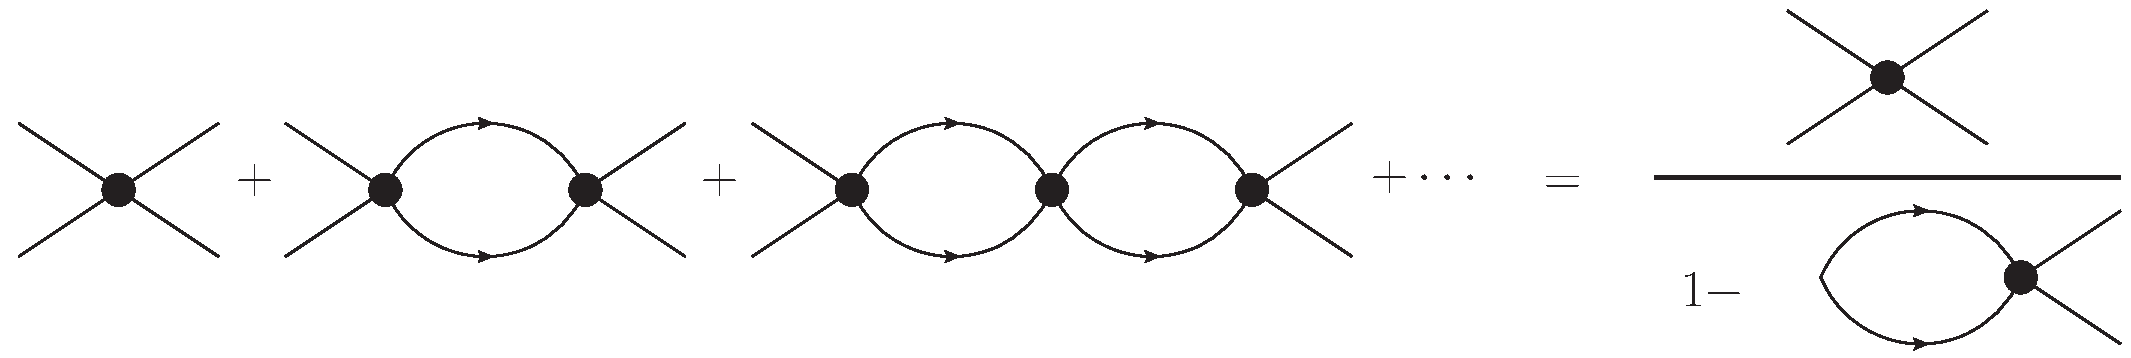
\includegraphics[width=\columnwidth]{figure/bubbleSum.pdf}
\caption{Bubble sum. Each line represents a propagator, each vertex represents $-i \sum_n C_{2n}(\Lambda) p^{2n}$, and the bubble is given by $I_0$ (see also \Figref{I0}).\label{fig:bubbleSum}}
\end{figure}

This bubble sum is a geometric series and gives, for the standard $T$-matrix, \cite{Kaplan:1998we,Beane:2003da}
\begin{equation}\label{eq:T matrix}
iT(p) = \frac{-i\sum_n C_{2n}(\Lambda) p^{2n}}{1-I_0(p,\Lambda) \sum_n C_{2n}(\Lambda) p^{2n}},
\end{equation}
where $p$ is the relative momentum,  and $I_0(p,\Lambda)$ is a $D$-dependent function that arises from integrating the loop shown in \Figref{I0},
\begin{align}
    I_0(p)
    &=-i\int^{\Lambda}
        \frac { \mathrm {d}q_0}{2\pi}\ \frac{\mathrm { d } ^ { D } \vec{ q } } { (2\pi)^ { D } }
        \left( \frac { i } { \frac{E}{2} + q _ { 0 } - \frac{\vec{q}^2}{2m_1} + i \epsilon } \right)
        \left( \frac { i } { \frac{E}{2} - q _ { 0 } - \frac{\vec{q}^2}{2m_2} + i \epsilon } \right)
    \label{eq:I0 in two particle language}\\
    &=\frac{\Omega_D}{(2\pi)^D}\int^{\Lambda}  \mathrm { d } q \ q^{D-1}\left[\PV \left( \frac { 1 } { E - \frac{\vec{q}^2}{2\mu} } \right)
-i\frac{\pi \mu}{q}\delta(q-\sqrt{2 \mu E})\right]
    \\
    &=\frac{\Omega_D}{(2\pi)^2}\frac{2\mu}{L^{D-2}}\int^{\Lambda L/2\pi}  \mathrm { d } n \ n^{D-1}\left[\PV \left( \frac { 1 } { \left(\frac{pL}{2\pi}\right)^2 - n^2 } \right)
-i\frac{\pi^2}{L n}\delta\left(\frac{2\pi}{L}n -p\right)\right]
    \label{eq:I0}
\end{align}
where $\PV$ refers to Principal (Cauchy) Value, we have used the on-shell condition $2\mu E=p^2$, and the geometric factor
\begin{equation}
\Omega_D=\frac{2\pi^{D/2}}{\Gamma(D/2)}=
    \begin{cases}
        4\pi    &   (D=3)\\
        2\pi    &   (D=2)\\
        2       &   (D=1)
    \end{cases}\ ,
\end{equation}
accounts for the angular integration in $D$ dimensions.

\begin{figure}[h!]
    \center
    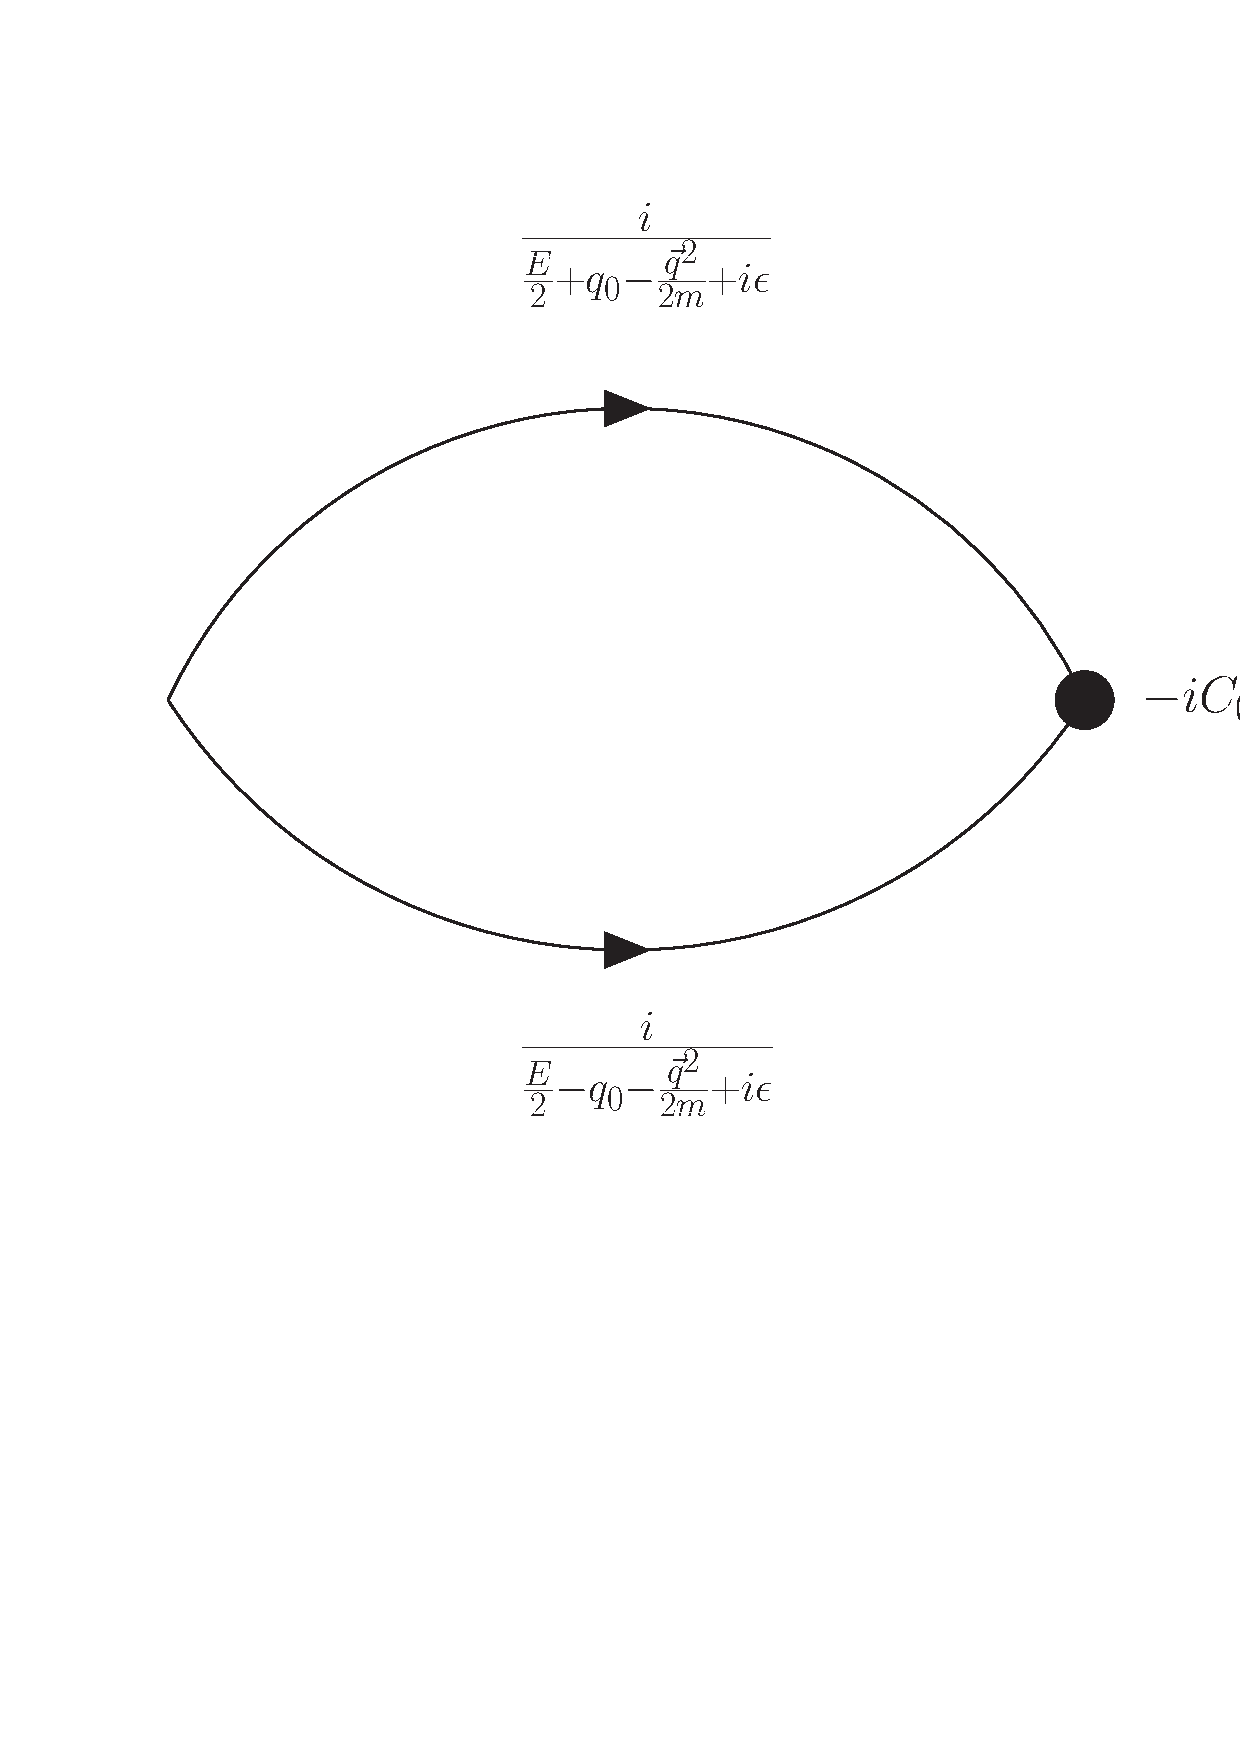
\includegraphics[width=.5\columnwidth]{figure/I0.pdf}
    \caption{
        Loop diagram contributing to the bubble sum.
    }
    \label{fig:I0}
\end{figure}

In the $s$-wave, the momentum-dependent $T$-matrix is related to the phase shift $\delta_0(p)$ by
\begin{equation}\label{eq:cot delta}
    i T = \frac{2}{\mu}\F_d\frac{i}{\cot \delta_0(p)-i}\ ,
\end{equation}
where
\begin{equation}\label{eq:spherical FD}
    \F_D
    =
    \begin{cases}
        \pi/p   & (D=3)\\
        1       & (D=2)\\
        p/2     & (D=1)
\end{cases}
\end{equation}
is a dimension-dependent kinematic factor.
This fixes the coefficients $C(\Lambda)$ as a function of the scattering data,
\begin{equation}\label{eq:IV pole}
    \frac{1}{\sum_n C_{2n}(\Lambda) p^{2n}}
    =
    I_0(p) - \frac{\mu}{2 \F_D}\left(\cot \delta_0(p) - i\right)
\end{equation}

In a finite volume, the energy eigenstates $E$ appear at poles of the $T$-matrix, so that
\begin{equation}\label{eq:FV pole}
    \frac{1}{\sum_n C_{2n}(\Lambda) \gamma^{2n}} - I_{0,\FV}(\gamma,L) = 0 \, ,
    \qquad
    \gamma^2 = 2 \mu E\, ,
\end{equation}
and the infinite-volume integral $I_0$ has been replaced by the matching finite-volume sum,
\begin{align}
I_{0,\FV}(\gamma,L)
    &=-i\int \frac { \mathrm {d}q_0}{2\pi} \frac{1}{L^D}\sum_{\vec{q}}^{q < \Lambda} \left( \frac { i } { \frac{E}{2} + q _ { 0 } - \frac{\vec{q}^2}{2m_1} + i \epsilon } \right) \left( \frac { i } { \frac{E}{2} - q _ { 0 } - \frac{\vec{q}^2}{2m_2} + i \epsilon } \right)
    \\
    &=\frac{1}{L^D}\sum_{\vec{q}}^{q < \Lambda} \frac { 1 } { E - \frac{\vec{q}^2}{2\mu} }
    =\frac{2\mu}{(2\pi)^2 L^{D-2}} \sum_{\vec{n}}^{n < \frac{\Lambda L}{2\pi}} \frac{1}{x-n^2}
    &
    x &= \left( \frac{\gamma L}{2\pi}\right)^2
    \, .
\end{align}
Combining the infinite-volume and finite-volume relations \eqref{IV pole} and \eqref{FV pole} yields
\begin{equation}\label{eq:spherical zeta}
    \frac{\mu}{2\F_D}(\cot\delta_0(\gamma)-i) = I_0(\gamma) - I_{0,\FV}(\gamma),
\end{equation}
the finite-volume quantization condition.
Note that both equations are explicitly evaluated for the same interactions using the same regulator and furthermore \eqref{spherical zeta} is only valid if evaluated at momenta $\gamma$ corresponding to FV eigenenergies $E$.

Plugging our results for the integrals in, one finds
\begin{equation}
    \frac{1}{2\F_D}\left(\cot \delta_0(\gamma) - i\right) = \frac{2}{(2\pi)^2 L^{D-2}}\left[ \left(\int_{\vec{n}} - \sum_{\vec{n}}\right) \frac{1}{x-n^2} + \frac{-i \pi^2\Omega_D}{L} \int \mathrm{d}n\ n^{D-2} \delta\left(\frac{2\pi}{L}n - \gamma\right) \right]
\end{equation}
where both the sum and integral are cut off by a restriction on the magnitude of $n$, $n^2 < (\Lambda L / 2\pi)^2$, and the integral implicitly carries a factor of $\Omega_D n^{D-1}$.
In a seemingly miraculous (but required) cancellation, the imaginary part on the left hand side exactly cancels the last term in the sum on the right,\footnote{Actually, the cancellation is not \emph{so} miraculous---demanding it occur is essentially how $\F_D$ is determined.} and we are left with
\begin{equation}
    \cot \delta_0(p) = \frac{\F_D}{\pi^2 L^{D-2}} \left(\sum_{\vec{n}}-\int_{\vec{n}}\right) \frac{1}{n^2-x}
\end{equation}
where $x=(\gamma L/2\pi)^2$ and we switched the sign of the sum and integral as well as the sign of the denominator.
Because we cut off the sum and the integral in exactly the same way, in dimensions where $I_0$ diverges with $\Lambda$, the divergence cancels against the divergence in the sum.
Let $N=\Lambda L/\pi$.
Then, defining, with a finite cutoff on magnitude $N/2$,
\begin{equation}\label{eq:spherical cutoff S}
    S^{\spherical N}_D(x) = \left(\sum_{\vec{n}}- \int_{\vec{n}}\right) \frac{1}{n^2-x}
\end{equation}
where the $\spherical$ superscript reminds us that we cut off our sum and integral in a spherical way, based on the magnitude of $n<N/2$, we recover the usual \Luscher zeta functions by taking
\begin{equation}\label{eq:spherical S}
    S^\spherical_D(x)
    =
    \lim_{N\goesto\infty} S^{\spherical N}_D(x)
    =
    \lim_{N\rightarrow\infty}\left( \sum_{\vec{n}}^{n < N/2} \frac{1}{n^2-x} - \counterterm_D^\spherical \left(\frac{N}{2}\right)^{D-2}\right)
\end{equation}
where dimension-dependent counterterm $\counterterm_D^\spherical$ comes from the integral; we evaluate the spherical-cutoff integrals and extract said counterterms in \Appref{counterterm/spherical}.
Finally,
\begin{equation}\label{eq:spherical quantization}
    \cot \delta_0(\gamma) = \frac{\F_D}{\pi^2 L^{D-2}} S^\spherical_D(x).
\end{equation}
This is the usual \Luscher finite-volume quantization condition, and continuum-extrapolated energy levels should be fed through it to produce continuum-limit scattering data.
In three dimensions it is common to move the momentum dependence in $\F_D$ to the other side, as $p \cot\delta_0(p)$ is what appears in the effective range expansion, as we will discuss in \Secref{ere}.

\subsection{Numerical Results}

Now we can attempt a numerical characterization of {\color{red} two} fermions at unitarity.
The interaction strength $C(\epsilon)$ of the Hamiltonian \eqref{p space hamiltonian}, in a three-dimensional cubic box of linear size $L$ with lattice spacing $\epsilon$, is tuned such that the ground state energy $E_0$ matches the first zero of $S^{\spherical}_3$.
The zeta function is evaluated using software provided by \Refs{Morningstar:2017spu,Morningstar:2hib}.
Once the strength is tuned to machine precision, using exact diagonalization we extract the low-lying energy levels, for fixed physical volume and fixed lattice spacing.
In \Figref{unimproved spherical} we put those (finite-lattice-spacing) energy levels through \eqref{spherical quantization} to convert them to scattering data, and additionally perform a continuum extrapolation according to
\begin{equation}
    \text{\todo{Does the extrapolation depend on \nstep?}}
\end{equation}
with error bars given by \todo{something meaningful}.  \todo{Add continuum extrapolation as an appendix?  Collect data, provide a script?  Something!}

\begin{figure}[th]
    \input{figure/ere-contact-fitted_a-inv_+0.0_zeta_spherical_projector_a1g_n-eigs_200.pgf}
    \caption{We show the result of tuning the contact interaction so that the ground state matches the first zero of $S^{\spherical}_3$.  In the top row we show results for $L=1.0$~fm, in bottom we show $L=2.0$~fm, while in different columns we show different finite differences as described in \eqref{p space hamiltonian}, \eqref{gamma definition}, and \eqref{gamma determination}. \todo{WHAT DO THESE UNITS MEAN?  I would advocate just making things non-dimensional by using factors of $m$ or something?}}
    \label{fig:unimproved spherical}
\end{figure}

\begin{figure}[th]
    \input{figure/continuum-ere_a-inv_+0.0_zeta_spherical_projector_a1g_n-eigs_200.pgf}
    \caption{Same as \Figref{unimproved spherical} but spectrum was extrapolated to continuum before fed to zeta function.}
    \label{fig:unimproved spherical continuum extrapolation}
\end{figure}

One can clearly see that without a continuum extrapolation, the finite-volume spectrum does not agree with the exactly-known flat solution that a contact interaction must provide.
That is, by foregoing a continuum extrapolation, we induce unphysical effects in the phase shift.
In the remainder of this paper we improve this result markedly, so that the continuum limit towards unitarity is substantially easier.

\todo{Comment on the continuum-extrapolated results, which I can't do yet since they're not there :D}

In \Figref{finite a spherical} we show the result of tuning the contact interaction so that the ground state, when put through $S^{\spherical}_3$ yields a scattering length of \todo{something}.
Again, since the interaction is a contact interaction only, we expect a completely flat behavior.
In constrast, we see \todo{shapes that make us sad / curious}.

\begin{figure}[th]
    \input{figure/ere-contact-fitted_a-inv_-5.0_zeta_spherical_projector_a1g_n-eigs_200.pgf}
    \caption{We results like \Figref{unimproved spherical}, but where the contact interaction was tuned so that the ground state matches yields $p\cot\delta = $\todo{some finite scattering length; part of \issue{19}} rather than to 0.  Similar deviation from completely flat behavior is apparent at any finite lattice spacing.}
    \label{fig:finite a spherical}
\end{figure}
